\documentclass[a4paper]{report}
\usepackage[utf8]{inputenc}
\usepackage[T1]{fontenc}
\usepackage{RJournal}
\usepackage{amsmath,amssymb,array}
\usepackage{booktabs}


% tightlist command for lists without linebreak
\providecommand{\tightlist}{%
  \setlength{\itemsep}{0pt}\setlength{\parskip}{0pt}}


% Always define CSL refs as bib entries are contained in separate doc
% Pandoc citation processing
\newlength{\cslhangindent}
\setlength{\cslhangindent}{1.5em}
\newlength{\csllabelwidth}
\setlength{\csllabelwidth}{3em}
\newlength{\cslentryspacingunit} % times entry-spacing
\setlength{\cslentryspacingunit}{\parskip}
% for Pandoc 2.8 to 2.10.1
\newenvironment{cslreferences}%
  {}%
  {\par}
% For Pandoc 2.11+
\newenvironment{CSLReferences}[2] % #1 hanging-ident, #2 entry spacing
 {% don't indent paragraphs
  \setlength{\parindent}{0pt}
  % turn on hanging indent if param 1 is 1
  \ifodd #1
  \let\oldpar\par
  \def\par{\hangindent=\cslhangindent\oldpar}
  \fi
  % set entry spacing
  \setlength{\parskip}{#2\cslentryspacingunit}
 }%
 {}
\usepackage{calc}
\newcommand{\CSLBlock}[1]{#1\hfill\break}
\newcommand{\CSLLeftMargin}[1]{\parbox[t]{\csllabelwidth}{#1}}
\newcommand{\CSLRightInline}[1]{\parbox[t]{\linewidth - \csllabelwidth}{#1}\break}
\newcommand{\CSLIndent}[1]{\hspace{\cslhangindent}#1}



\begin{document}


%% do not edit, for illustration only
\sectionhead{Contributed research article}
\volume{XX}
\volnumber{YY}
\year{20ZZ}
\month{AAAA}

\begin{article}
  % !TeX root = RJwrapper.tex
\title{Computer Algebra in \texttt{R} Bridges a Gap Between Mathematics and Data in the Teaching of Statistics and Data Science}
\author{by Mikkel Meyer Andersen and Søren Højsgaard}

\maketitle

\abstract{%
The capability of R to do symbolic mathematics is enhanced by the \texttt{caracas} package. This package uses the Python computer algebra library SymPy as a back-end but \texttt{caracas} is tightly integrated in the R environment, thereby enabling the R user with symbolic mathematics within R. We demonstrate how mathematics and statistics can benefit from bridging computer algebra and data via R. This is done thought a number of examples and we propose some topics for small student projects. The \texttt{caracas} package integrates well with e.g.~\texttt{Rmarkdown}, and as such creation of scientific reports and teaching is supported.
}

\hypertarget{introduction}{%
\section{Introduction}\label{introduction}}

The \CRANpkg{caracas} package (Andersen and Højsgaard 2021) and the \CRANpkg{Ryacas}
package (Andersen and Højsgaard 2019) enhance the capability of \texttt{R} (R Core Team 2023) to handle
symbolic mathematics. In this paper we will illustrate the use of the
\texttt{caracas} package in connection with teaching mathematics and
statistics. Focus is on 1) treating statistical models symbolically,
2) on bridging the gap between symbolic mathematics and numerical
computations and 3) on preparing teaching material in a reproducible
framework (provided by, e.g.~\CRANpkg{rmarkdown} (Allaire et al. 2021; Xie, Allaire, and Grolemund 2018; Xie, Dervieux, and Riederer 2020)). The \texttt{caracas} package
is available from CRAN (R Core Team 2023). The open-source development version of
\texttt{caracas} is available at \url{https://github.com/r-cas/caracas} and
readers are recommended to study the online documentation at
\url{https://r-cas.github.io/caracas/}. The \texttt{caracas} package provides an
interface from \texttt{R} to the \texttt{Python} package \texttt{sympy} (Meurer et al. 2017). This
means that SymPy is ``running under the hood'' of \texttt{R} via the
\texttt{reticulate} package (Ushey, Allaire, and Tang 2020). The \texttt{sympy} package is mature and
robust with many users and developers.

Neither \texttt{caracas} nor \texttt{Ryacas} are as powerful as some
of the larger commercial computer algebra systems (CAS). The virtue of
\texttt{caracas} and \texttt{Ryacas} lie elsewhere:
(1) Mathematical tools like equation solving, summation, limits, symbolic linear
algebra, outputting in tex format etc. are directly available from
within \texttt{R}.
(2) The packages enable working with the same language and in the same
environment as the user does for statistical analyses.
(3) Symbolic mathematics can easily be combined with data which is
helpful in e.g.~numerical optimization.
(4) The packages are open-source and therefore support e.g.~education - also for people
with limited economical means and thus contributing to United
Nations sustainable development goals (United Nations General Assembly 2015).

The paper is organized in the following sections: The section
{[}Mathematics and documents containing mathematics{]} briefly introduces
the \texttt{caracas} package and its syntax, including how \texttt{caracas} can be
used in connection with preparing texts, e.g.~teaching material. More
details are provided in the Section {[}Important technical aspects{]}.
Several vignettes illustrating \texttt{caracas} are provided and they are
also available online, see \url{https://r-cas.github.io/caracas/}. The
section \protect\hyperlink{statistics-examples}{Statistics examples} is the main section of the paper and
here we present a sample of statistical models where we believe that a
symbolic treatment is a valuable supplement to a numerical in
connection with teaching. The section {[}Possible topics to study{]}
contains suggestions about hand-on activities for students. Lastly,
the section \protect\hyperlink{discussion-and-future-work}{Discussion and future work} contains a discussion of the
paper.

\hypertarget{using-caracas-better-title}{%
\section{\texorpdfstring{Using \texttt{caracas} {[}Better title{]}}{Using caracas {[}Better title{]}}}\label{using-caracas-better-title}}

Introduce key concepts and show functionality subsequently needed in the section \protect\hyperlink{statistics-examples}{Statistics examples}.

\hypertarget{symbols}{%
\subsection{Symbols}\label{symbols}}

A \texttt{caracas} symbol is a list with a \texttt{pyobj} slot and the class
\texttt{caracas\_symbol}. The \texttt{pyobj} is an object in \texttt{Python} (often a
\texttt{sympy} object). As such, a symbol (in \texttt{R}) provides a handle to a
\texttt{Python} object. In the design of \texttt{caracas} we have tried to make
this distinction something the user should not be concerned with, but
it is worthwhile being aware of the distinction.
Symbols can be created with \texttt{def\_sym()} and \texttt{as\_sym()}. Both declares
the symbol in \texttt{R} and in \texttt{Python}.

\hypertarget{documents-with-mathematical-content}{%
\subsection{Documents with mathematical content}\label{documents-with-mathematical-content}}

A LaTeX rendering of a \texttt{caracas} symbol, say \texttt{x} is obtained by typing
\texttt{\$\$x\ =\ \textasciigrave{}r\ tex(x)\textasciigrave{}\$\$}. This feature is useful when creating documents with a mathematical content and has been used extensively throughout this paper (looks nice and saves space).

\hypertarget{linear-algebra}{%
\subsection{Linear algebra}\label{linear-algebra}}

We create a symbolic matrix and find its inverse:

\begin{verbatim}
R> M0 <- toeplitz(c("a", "b")) ## Character matrix
R> M <- as_sym(M0)                ## as_sym() converts to a caracas symbol
R> Minv <- inv(M) %>% simplify()
\end{verbatim}

Default printing of \texttt{M} is:

\begin{verbatim}
R> M
\end{verbatim}

\begin{verbatim}
#> [c]: [a  b]
#>      [    ]
#>      [b  a]
\end{verbatim}

The determinant of \(M\), \(det(M)=a^2 - b^2\), can be factored out of
the matrix by dividing each entry with the determinant and multiplying
the new matrix by the determinant which simplifies the appearance of
the matrix:

\begin{verbatim}
R> Minv_fact <- as_factor_list(1 / factor_(det(M)), simplify(Minv * det(M)))
\end{verbatim}

Hence we have in LaTeX format:

\[
M = \left[\begin{matrix}a & b\\b & a\end{matrix}\right]; \quad M^{-1} = \frac{1}{\left(a - b\right) \left(a + b\right)}  \left[\begin{matrix}a & - b\\- b & a\end{matrix}\right] = \left[\begin{matrix}\frac{a}{a^{2} - b^{2}} & - \frac{b}{a^{2} - b^{2}}\\- \frac{b}{a^{2} - b^{2}} & \frac{a}{a^{2} - b^{2}}\end{matrix}\right] .
\]

A \texttt{caracas} symbol can be coerced to an \texttt{R} expression
using \texttt{as\_expr()}.
Symbols can be substituted with other symbols or with numerical values
using \texttt{subs()}:

\begin{verbatim}
R> as_expr(M)
\end{verbatim}

\begin{verbatim}
#> expression(matrix(c(a, b, b, a), nrow = 2))
\end{verbatim}

\begin{verbatim}
R> def_sym(a) ## FIXME: Should this be necessary
R> M2 <- subs(M, "b", "a^2")
R> M3 <- subs(M2, a, 2)
\end{verbatim}

\[
M2 = \left[\begin{matrix}a & a^{2}\\a^{2} & a\end{matrix}\right]; \quad
M3 = \left[\begin{matrix}2 & 4\\4 & 2\end{matrix}\right]; \quad
\]

A vector is a one-column matrix which is printed as its transpose to save space. Matrix products are computed using the \texttt{\%*\%} operator:

\begin{verbatim}
R> v <- vector_sym(2, "v")
R> Mv <- M %*% v
\end{verbatim}

\[
v = \left[\begin{matrix}v_{1}\\v_{2}\end{matrix}\right]; \quad  Mv = \left[\begin{matrix}a v_{1} + b v_{2}\\a v_{2} + b v_{1}\end{matrix}\right]
\]

\hypertarget{calculus}{%
\subsection{Calculus}\label{calculus}}

Next, we define a \texttt{caracas} symbol \texttt{x} and
subsequently a \texttt{caracas} polynomial \texttt{p} in \texttt{x} (\texttt{p} becomes a symbol because \texttt{x} is):

\begin{verbatim}
R> library(caracas)
R> def_sym(x) ## Declares 'x' as a symbol
R> p <- 1 - x^2 + x^3 + x^4/4 - 3 * x^5 / 5 + x^6 / 6
\end{verbatim}

\[
x = x; \quad p = \frac{x^{6}}{6} - \frac{3 x^{5}}{5} + \frac{x^{4}}{4} + x^{3} - x^{2} + 1
\]

Note that \texttt{x} exists in both \texttt{R} and \texttt{Python}, whereas \texttt{p}
exists only as a caracas symbol in R; there is no corresponding object
\texttt{p} in Python:

\begin{verbatim}
R> x$pyobj
\end{verbatim}

\begin{verbatim}
#> x
\end{verbatim}

\begin{verbatim}
R> p$pyobj
\end{verbatim}

\begin{verbatim}
#> x**6/6 - 3*x**5/5 + x**4/4 + x**3 - x**2 + 1
\end{verbatim}

We investigate \texttt{p} further by finding the gradient and Hessian of \texttt{p}. The gradient factors which shows that the stationary
points are \(-1\), \(0\), \(1\) and \(2\).

\begin{verbatim}
R> grad <- der(p, x) 
R> grad2 <- factor_(grad)
R> hess <- der2(p, x)
\end{verbatim}

\[
 grad  = x^{5} - 3 x^{4} + x^{3} + 3 x^{2} - 2 x; \quad 
 grad2  = x \left(x - 2\right) \left(x - 1\right)^{2} \left(x + 1\right); \quad  
\]

In a more general setting we can find the stationary points by equating the gradient to zero:
The output \texttt{sol} is a list of list of \texttt{caracas} symbols.

\begin{verbatim}
R> sol <- solve_sys(lhs = grad, rhs=0, vars = x) 
R> sol_expr <- sapply(sol, sapply, as_expr) |> unname()
R> sol_expr
\end{verbatim}

\begin{verbatim}
#> [1] -1  0  1  2
\end{verbatim}

A \texttt{caracas} symbol can be turned into an \texttt{R} function for subsequent
numerical evaluation using \texttt{as\_func()}, see
Fig. \ref{fig:calculus}.
The stationary points are indicated in the plots.

\begin{verbatim}
R> p_fn <- as_func(p)
R> p_fn
\end{verbatim}

\begin{verbatim}
#> function(x)
#> { 
#> x^6/6 - 3 * x^5/5 + x^4/4 + x^3 - x^2 + 1
#> }
#> <environment: 0x55c36ba691b0>
\end{verbatim}

\begin{verbatim}
R> grad_fn <- as_func(grad)
R> hess_fn <- as_func(hess)
R> hess_fn(sol_expr)
\end{verbatim}

\begin{verbatim}
#> [1] 12 -2  0  6
\end{verbatim}

The sign of the Hessian in the stationary
points show \(-1\) and \(2\) are local minima, \(0\) is a local maximum and
\(1\) is an inflection point.

\begin{figure}
\centering
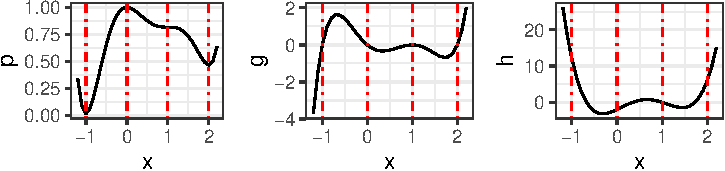
\includegraphics{paper-r00_files/figure-latex/calculus-1.pdf}
\caption{\label{fig:calculus}Left: A polynomium. Center: The gradient. Right: The Hessian.}
\end{figure}

\hypertarget{integration}{%
\subsection{Integration}\label{integration}}

The unit circle is given by \(x^2 + y^2 = 1\) so the area of the upper
half of the unit circle is \(\int_{-1}^1 \sqrt{1-x^2}dx\) (which is
known to be \(\pi/2\)). This result is produced by \texttt{caracas} while the
\texttt{integrate} function in \texttt{R} produces the approximate result \(1.57\).

\begin{verbatim}
R> x <- as_sym("x")
R> half_circle_ <- sqrt(1-x^2)
R> ## Anti derivative:
R> ad <- int(half_circle_, "x")
R> ## Definite integral:
R> di <- int(half_circle_, "x", -1, 1)
\end{verbatim}

\[
ad = \frac{x \sqrt{1 - x^{2}}}{2} + \frac{\operatorname{asin}{\left(x \right)}}{2} \quad
di = \frac{\pi}{2}
\]

\hypertarget{unevaluated-expressions}{%
\subsection{Unevaluated expressions}\label{unevaluated-expressions}}

Finally we illustrate creation of unevaluated expressions:

\begin{verbatim}
R> def_sym(x, n)
R> y <- (1 + x/n)^n
R> l <- lim(y, n, Inf, doit = FALSE)
R> l2 <- doit(l)
\end{verbatim}

\[
l = \lim_{n \to \infty} \left(1 + \frac{x}{n}\right)^{n}; \quad l2 = e^{x}
\]

Several functions have the \texttt{doit} argument, e.g.~\texttt{lim()}, \texttt{int()} and \texttt{sum\_()}.
That helps making reproducible documents where the changes
in code appears automatically in the generated formulas.

\hypertarget{statistics-examples}{%
\section{Statistics examples}\label{statistics-examples}}

In this section we examine larger statistical examples and
demonstrate how \texttt{caracas} can help improve understanding of the models.

\hypertarget{example-linear-models}{%
\subsection{Example: Linear models}\label{example-linear-models}}

A matrix algebra approach to e.g.~linear models is very clear and
concise. On the other hand, it can also be argued that matrix algebra
obscures what is being computed. Numerical examples are useful for
some aspects of the computations but not for other. In this respect
symbolic computations can be enlightening.

Consider a two-way analysis of variance (ANOVA) with one observation
per group, see Table \ref{tab:anova-two-way-table}.

\begin{table}[!h]

\caption{\label{tab:anova-two-way-table}Two-by-two layout of data.}
\centering
\begin{tabular}[t]{|>{}l|>{}l|}
\hline
$y_{11}$ & $y_{21}$\\
\hline
$y_{12}$ & $y_{22}$\\
\hline
\end{tabular}
\end{table}

\begin{verbatim}
R> nr <- 2
R> nc <- 2
R> y <- matrix_sym(nr, nc, "y")
R> dim(y) <- c(nr * nc, 1)
R> y
\end{verbatim}

\begin{verbatim}
#> [c]: [y11  y21  y12  y22]^T
\end{verbatim}

\begin{verbatim}
R> dat <- expand.grid(r=factor(1:nr), s=factor(1:nc))
R> X <- model.matrix(~ r + s, data=dat) |> as_sym()
R> b <- vector_sym(ncol(X), "b")
R> mu <- X %*% b
\end{verbatim}

For the specific model we have random variables \(y=(y_{ij})\). All
\(y_{ij}\)s are assumed independent and \(y_{ij}\sim N(\mu_{ij}, v)\).
The corresponding mean vector \(\mu\) has the form given below:

\[
y = \left[\begin{matrix}y_{11}\\y_{21}\\y_{12}\\y_{22}\end{matrix}\right], \quad X=\left[\begin{matrix}1 & . & .\\1 & 1 & .\\1 & . & 1\\1 & 1 & 1\end{matrix}\right], \quad b=\left[\begin{matrix}b_{1}\\b_{2}\\b_{3}\end{matrix}\right], \quad  \mu = X b = \left[\begin{matrix}b_{1}\\b_{1} + b_{2}\\b_{1} + b_{3}\\b_{1} + b_{2} + b_{3}\end{matrix}\right] .
\]

Above and elsewhere, dots represent zero.
The least squares estimate of \(b\) is the vector \(\hat{b}\) that minimizes \(||y-X b||^2\) which leads to the normal equations \((X^\top X)b = X^\top y\) to be solved. If \(X\) has full rank, the unique solution to the normal
equations is \(\hat{b} = (X^\top X)^{-1} X^\top y\). Hence the
estimated mean vector is \(\hat \mu = X\hat{b}=X(X^\top X)^{-1} X^\top y\). Symbolic computations are
not needed for quantities involving only the model matrix \(X\), but
when it comes to computations involving \(y\), a symbolic treatment of
\(y\) is useful:

\begin{verbatim}
R> XtX <- t(X) %*% X
R> XtXinv <- inv(XtX)
R> Xty <- t(X) %*% y
R> b_hat <- XtXinv %*% Xty
\end{verbatim}

\begin{align}
X^\top y &= \left[\begin{matrix}y_{11} + y_{12} + y_{21} + y_{22}\\y_{21} + y_{22}\\y_{12} + y_{22}\end{matrix}\right] , 
\quad
\hat{b} = \frac{1}{4}  \left[\begin{matrix}3 y_{11} + y_{12} + y_{21} - y_{22}\\- 2 y_{11} - 2 y_{12} + 2 y_{21} + 2 y_{22}\\- 2 y_{11} + 2 y_{12} - 2 y_{21} + 2 y_{22}\end{matrix}\right]
\end{align}

Hence \(X^\top y\) (a sufficient reduction of data if the variance is known)
consists of the sum of all observations, the sum of
observations in the second row and the sum of observations in the second column. For \(\hat{b}\), the second component is, apart from a scaling, the sum of the second row minus the sum of the first row. Likewise, the third component is the sum of the second column minus the sum of the first column. It is hard to give an interpretation of the first component of \(\hat{b}\).

\hypertarget{example-logistic-regression}{%
\subsection{Example: Logistic regression}\label{example-logistic-regression}}

In the following we go through details of a logistic regression model,
see e.g.~McCullagh and Nelder (1989) for a classical description of logistic
regression: Observables are binomially distributed, \(y_i \sim \text{bin}(p_i, n_i)\). The probability \(p_i\) is connected to a
\(q\)-vector of covariates \(x_i=(x_{i1}, \dots, x_{iq})\) and a
\(q\)-vector of regression coefficients \(b=(b_1, \dots, b_q)\) as
follows: The term \(s_i = x_i \cdot b\) is denoted the \emph{linear
predictor}. The probability \(p_i\) can be linked to \(s_i\) in different
ways, but the most commonly employed is via the \emph{logit link
function} which is \(\text{logit}(p_i) = \log(p_i/(1-p_i))\) so here
\(\text{logit}(p_i) = s_i\).

As an example, consider the \texttt{budworm} data from the \CRANpkg{doBy} package (Højsgaard and Halekoh 2023).
The data shows the number of killed moth tobacco budworm
\emph{Heliothis virescens}. Batches of 20 moths of each sex were
exposed for three days to the pyrethroid and the number in each batch
that were dead or knocked down was recorded:

\begin{verbatim}
R> data(budworm, package = "doBy")
R> bud <- subset(budworm, sex == "male")
R> bud
\end{verbatim}

\begin{verbatim}
#>    sex dose ndead ntotal
#> 1 male    1     1     20
#> 2 male    2     4     20
#> 3 male    4     9     20
#> 4 male    8    13     20
#> 5 male   16    18     20
#> 6 male   32    20     20
\end{verbatim}

Below we focus only on male budworms and the mortality is illustrated
in Figure \ref{fig:budworm} (produced with \CRANpkg{ggplot2} (Wickham 2016)). On the \(y\)-axis we have the empirical
logits, i.e.~\(\log((\text{ndead} + 0.5)/(\text{ntotal}-\text{ndead} + 0.5))\). The figure suggests that logit grows linearly with log dose.

\begin{figure}
\centering
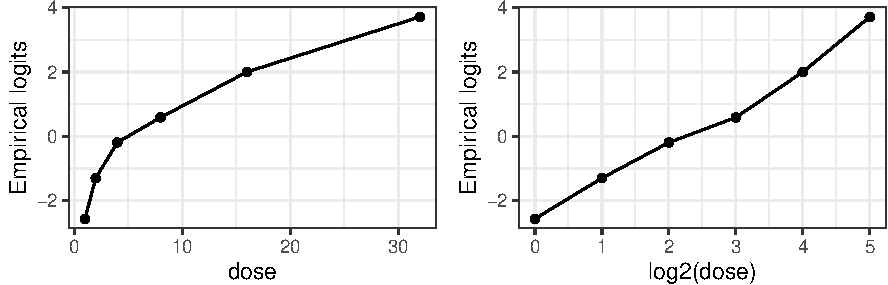
\includegraphics{paper-r00_files/figure-latex/budworm-1.pdf}
\caption{\label{fig:budworm}Insecticide mortality of the moth tobacco budworm.}
\end{figure}

\hypertarget{each-component-of-the-likelihood}{%
\subsubsection{Each component of the likelihood}\label{each-component-of-the-likelihood}}

The log-likelihood is \(\log L=\sum_i y_i \log(p_i) + (n_i-y_i) \log(1-p_i) = \sum_i \log L_i\), say. With \(\log(p_i/(1-p_i)) = s_i\) we
have \(p_i=1 / (1+ \exp(-s_i))\) and \(\frac d {ds_i} p_i = \frac{\exp(- s_i)}{\left(1 + \exp(- s_i)\right)^{2}}\). With \(s_i = x_i\cdot b\), we
have \(\frac d {db} s_i = x_i\).

Consider the contribution to the total log-likelihood from the \(i\)th
observation which is \(l_i = y_i \log(p_i) + (n_i-y_i) \log(1-p_i)\).
Since we are focusing on one observation only, we shall ignore the
subscript \(i\) in this section. First notice that with
\(s = \log(p/(1-p))\) we can find \(p\) as:

\begin{verbatim}
R> def_sym(s, p)
R> sol_ <- solve_sys(lhs = log(p / (1 - p)), rhs = s, vars = p)
R> sol_[[1]]$p
\end{verbatim}

\begin{verbatim}
#> [c]:   exp(s)  
#>      ----------
#>      exp(s) + 1
\end{verbatim}

Next, find the likelihood as a function of \(p\), as a function of \(s\) and as a function of \(b\).
The underscore in \texttt{logLb\_} and elsewhere indicates that this expression
is defined in terms of other symbols (this is in contrast
to the free variables, e.g.~\texttt{y}, \texttt{p}, and \texttt{n}.):

\begin{verbatim}
R> def_sym(y, n, p, x, s, b)
R> logLp_ <- y * log(p) + (n - y) * log(1 - p)
R> p_ <- exp(s) / (exp(s) + 1)
R> logLs_ <- subs(logLp_, p, p_)
R> s_ <- sum(x * b)
R> logLb_ <- subs(logLs_, s, s_)
R> logLb_
\end{verbatim}

\begin{verbatim}
#> [c]:      /  exp(b*x)  \              /      exp(b*x)  \
#>      y*log|------------| + (n - y)*log|1 - ------------|
#>           \exp(b*x) + 1/              \    exp(b*x) + 1/
\end{verbatim}

The log-likelihood can be maximized using e.g.~Newton-Rapson (see e.g.~Nocedal and Wright (2006)) and in this connection we
need the score function, \(S\), and the Hessian, \(H\):

\begin{verbatim}
R> Sb_ <- score(logLb_, b) |> simplify()
R> Hb_ <- hessian(logLb_, b) |> simplify()
R> Sb_
\end{verbatim}

\begin{verbatim}
#> [c]: [x*(y - (n - y)*exp(b*x))]
#>      [------------------------]
#>      [      exp(b*x) + 1      ]
\end{verbatim}

\begin{verbatim}
R> Hb_
\end{verbatim}

\begin{verbatim}
#> [c]: [          2                ]
#>      [      -n*x *exp(b*x)       ]
#>      [---------------------------]
#>      [exp(2*b*x) + 2*exp(b*x) + 1]
\end{verbatim}

Since \(x\) and \(b\) are vectors, the term \texttt{b*x} above should be read
as the inner product \(x \cdot b\) (or as \(x^\top b\) in matrix
notation). Also, since \(x\) is a vector, the term \texttt{x\^{}2} above should
be read as the outer product \(x \otimes x\) (or as \(x x^\top\) in
matrix notation). More insight in the structure is obtained by
letting \(b\) and \(x\) be \(2\)-vectors (to save space, the Hessian matrix is omitted in the following):

\begin{verbatim}
R> b <- vector_sym(2, "b")
R> x <- vector_sym(2, "x")
R> s_ <- sum(x * b)
R> logLb_ <- subs(logLs_, s, s_)
R> Sb_ <- score(logLb_, b) |> simplify()
\end{verbatim}

\begin{align}
\texttt{logLb}\_ &= y \log{\left(\frac{e^{b_{1} x_{1} + b_{2} x_{2}}}{e^{b_{1} x_{1} + b_{2} x_{2}} + 1} \right)} + \left(n - y\right) \log{\left(1 - \frac{e^{b_{1} x_{1} + b_{2} x_{2}}}{e^{b_{1} x_{1} + b_{2} x_{2}} + 1} \right)}, \\
\texttt{Sb}\_    &= \left[\begin{matrix}\frac{x_{1} \left(- n e^{b_{1} x_{1} + b_{2} x_{2}} + y e^{b_{1} x_{1} + b_{2} x_{2}} + y\right)}{e^{b_{1} x_{1} + b_{2} x_{2}} + 1}\\\frac{x_{2} \left(- n e^{b_{1} x_{1} + b_{2} x_{2}} + y e^{b_{1} x_{1} + b_{2} x_{2}} + y\right)}{e^{b_{1} x_{1} + b_{2} x_{2}} + 1}\end{matrix}\right] .
\end{align}

Next, insert data, e.g.~\(x_{1}=1\), \(x_{2}=2\), \(y=9\), \(n=20\) to obtain a function of the regression parameters only. Note how the expression depending on other symbols, \texttt{S\_}, is
named \texttt{S.} to indicate that data has been inserted:

\begin{verbatim}
R> nms <- c("x1", "x2", "y", "n")
R> vls <- c(1, 2, 9, 20)
R> logLb. <- subs(logLb_, nms, vls)
R> Sb. <- subs(Sb_, nms, vls)
\end{verbatim}

The total score for the entire dataset can be obtained as follows:

\begin{verbatim}
R> Sb_list <- lapply(seq_len(nrow(bud)), function(r){
+   vls <- c(1, log2(bud$dose[r]), bud$ndead[r], bud$ntotal[r])
+   subs(Sb_, nms, vls) 
+ })
R> Sb_total <- Reduce(`+`, Sb_list)
\end{verbatim}

This score can be used as part of an iterative algorithm for solving the score equations.
If one wants to use Newton-Rapson, the total Hessian matrix must also be created
following lines similar to those above.
It is straight forward implement a Newton-Rapson algorithm based on these
quantities, one must only note the distinction between the two expressions
below (and it is the latter one would use in an iterative algorithm):

\begin{verbatim}
R> subs(Sb_total, b, c(1, 2))
R> subs(Sb_total, b, c(1, 2)) |> as_expr()
\end{verbatim}

An alternative is to construct the total log-likelihood
for the entire dataset as a \texttt{caracas} object, convert this
object to an \texttt{R} function and maximize this
function using one of \texttt{R}'s optimization methods:

\begin{verbatim}
R> logLb_list <- lapply(seq_len(nrow(bud)), function(r){
+   vls <- c(1, log2(bud$dose[r]), bud$ndead[r], bud$ntotal[r])
+   subs(logLb_, nms, vls) 
+ })
R> logLb_total <- Reduce(`+`, logLb_list)
R> logLb_total_func <- as_func(logLb_total, vec_arg = TRUE)
\end{verbatim}

\hypertarget{the-total-likelihood-symbolically}{%
\subsubsection{The total likelihood symbolically}\label{the-total-likelihood-symbolically}}

We conclude this section by illustrating that the log-likelihood for the entire dataset
can be constructed in a few steps (output is omitted to save space):

\begin{verbatim}
R> X. <- as_sym(cbind(1, log2(bud$dose)))
R> n. <- as_sym(bud$ntotal)
R> y. <- as_sym(bud$ndead)
R> N <- nrow(X.)
R> q <- ncol(X.)
R> X <- matrix_sym(N, q, "x")
R> n <- vector_sym(N, "n")
R> y <- vector_sym(N, "y")
R> p <- vector_sym(N, "p")
R> s <- vector_sym(N, "s")
R> b <- vector_sym(q, "b")
\end{verbatim}

\[
 X=\left[\begin{matrix}x_{11} & x_{12}\\x_{21} & x_{22}\\x_{31} & x_{32}\\x_{41} & x_{42}\\x_{51} & x_{52}\\x_{61} & x_{62}\end{matrix}\right], \quad
 X.=\left[\begin{matrix}1 & 0\\1 & 1\\1 & 2\\1 & 3\\1 & 4\\1 & 5\end{matrix}\right], \quad
 n.=\left[\begin{matrix}20\\20\\20\\20\\20\\20\end{matrix}\right], \quad
 n=\left[\begin{matrix}n_{1}\\n_{2}\\n_{3}\\n_{4}\\n_{5}\\n_{6}\end{matrix}\right], \quad
 y.=\left[\begin{matrix}1\\4\\9\\13\\18\\20\end{matrix}\right] .
\]

The symbolic computations are as follows:

\begin{verbatim}
R> ## log-likelihood as function of p
R> logLp  <- sum(y * log(p) + (n-y) * log(1-p))
R> ## log-likelihood as function of s
R> p_ <- exp(s) / (exp(s) + 1)
R> logLs <- subs(logLp, p, p_)
R> ## linear predictor as function of regression coefficients:
R> s_  <- X %*% b
R> ## log-Likelihood as function of regression coefficients:
R> logLb <- subs(logLs, s, s_)
\end{verbatim}

Next, numerical values can be inserted:

\begin{verbatim}
R> logLb <- subs(logLb, cbind(n, y, X), cbind(n., y., X.))
\end{verbatim}

An alternative would have been to define \texttt{logLp} above in terms of
\texttt{n.} and \texttt{y.} and similarly define \texttt{s\_} in terms of \texttt{X.} If doing so,
the last step where numerical values are inserted could have been
avoided. From here, one may proceed by computing the score function
and the Hessian matrix and solve the score equation, using
e.g.~Newton-Rapson. Alternatively, one might create an \texttt{R} function
based on the log-likelihood, and maximize this function using one of
\texttt{R}'s optimization methods (see the example in the previous section):

\begin{verbatim}
R> logLb_func <- as_func(logLb, vec_arg = TRUE)
R> optim(c(0, 0), logLb_func, control = list(fnscale = -1), hessian = TRUE)
\end{verbatim}

\hypertarget{example-constrained-maximum-likelihood}{%
\subsection{Example: Constrained maximum likelihood}\label{example-constrained-maximum-likelihood}}

In this section we illustrate constrained optimization using Lagrange multipliers.
This is demonstrated for the independence model for a two-way contingency table.
Consider a \(2 \times 2\) contingency table with cell
counts \(y_{ij}\) and cell probabilities \(p_{ij}\) for \(i=1,2\) and \(j=1,2\),
where \(i\) refers to row and \(j\) to column as
illustrated in Table \ref{tab:anova-two-way-table}.

Under multinomial sampling, the log likelihood is
\[
 l = \log L = \sum_{ij} y_{ij} \log(p_{ij}).
\]

Under the assumption of independence between rows and columns, the cell
probabilities have the form, (see e.g.~Højsgaard, Edwards, and Lauritzen (2012), p.~32)
\[
p_{ij}=u \cdot r_i \cdot s_j.
\]

To make the parameters \((u, r_i, s_j)\) identifiable, constraints
must be imposed. One possibility is to require that \(r_1=s_1=1\). The
task is then to estimate \(u\), \(r_2\), \(s_2\) by maximizing the log likelihood
under the constraint that \(\sum_{ij} p_{ij} = 1\). This can be
achieved using a Lagrange multiplier where we instead solve the
unconstrained optimization problem \(\max_p Lag(p)\) where
\begin{align}
  Lag(p) &= -l(p) + \lambda g(p) \quad \text{under the constraint that} \\
  g(p) &= \sum_{ij} p_{ij} - 1 = 0 ,
\end{align}
where \(\lambda\) is a Lagrange multiplier.
In \texttt{SymPy}, \texttt{lambda} is a reserved symbol. Hence the underscore as postfix below:

\begin{verbatim}
R> y_ <- c("y_11", "y_21", "y_12", "y_22")
R> y  <- as_sym(y_)
R> def_sym(u, r2, s2, lambda_)
R> p <- as_sym(c("u", "u*r2", "u*s2", "u*r2*s2"))
R> logL  <- sum(y * log(p))
R> Lag  <- -logL + lambda_ * (sum(p) - 1) 
R> vars <- list(u, r2, s2, lambda_)
R> gLag <- der(Lag, vars)
R> sol <- solve_sys(gLag, vars)
R> print(sol, method = "ascii")
\end{verbatim}

\begin{verbatim}
#> Solution 1:
#>   u       =  (y_11 + y_12)*(y_11 + y_21)/(y_11 + y_12 + y_21 + y_22)^2 
#>   r2      =  (y_21 + y_22)/(y_11 + y_12) 
#>   s2      =  (y_12 + y_22)/(y_11 + y_21) 
#>   lambda_ =  y_11 + y_12 + y_21 + y_22
\end{verbatim}

\begin{verbatim}
R> sol <- sol[[1]]
\end{verbatim}

There is only one critical point. Fitted cell probabilities \(\hat p_{ij}\) are:

\begin{verbatim}
R> p11 <- sol$u
R> p21 <- sol$u * sol$r2
R> p12 <- sol$u * sol$s2
R> p22 <- sol$u * sol$r2 * sol$s2
R> p.hat <- matrix_(c(p11, p21, p12, p22), nrow = 2)
\end{verbatim}

\[
\hat p = \frac{1}{\left(y_{11} + y_{12} + y_{21} + y_{22}\right)^{2}}  \left[\begin{matrix}\left(y_{11} + y_{12}\right) \left(y_{11} + y_{21}\right) & \left(y_{11} + y_{12}\right) \left(y_{12} + y_{22}\right)\\\left(y_{11} + y_{21}\right) \left(y_{21} + y_{22}\right) & \left(y_{12} + y_{22}\right) \left(y_{21} + y_{22}\right)\end{matrix}\right]
\]

To verify that the maximum likelihood estimate has been found, we compute the Hessian matrix
which is negative definite (the Hessian matrix is diagonal so the eigenvalues are the diagonal entries and these are all negative), output omitted:

\begin{verbatim}
R> H <- hessian(logL, list(u, r2, s2)) |> simplify()
\end{verbatim}

\hypertarget{example-an-auto-regression-model}{%
\subsection{Example: An auto regression model}\label{example-an-auto-regression-model}}

\hypertarget{symbolic-computations}{%
\subsubsection{Symbolic computations}\label{symbolic-computations}}

In this section we study the auto regressive model of order \(1\) (an AR(1) model), see
e.g.~Shumway and Stoffer (2016), p.~75 ff.~for details:
Consider random variables \(x_1, x_2, \dots, x_n\) following a stationary zero mean AR(1) process:

\begin{equation}
  x_i = a x_{i-1} + e_i; \quad i=2, \dots, n,
  \label{eq:ar1}
\end{equation}

where \(e_i \sim N(0, v)\) and all \(e_i\)s are independent. Note that \(v\) denotes the variance.
The marginal distribution of \(x_1\) is also assumed normal, and for the process to be stationary
we must have that the variance \(\mathbf{Var}(x_1) = v / (1-a^2)\).
Hence we can write \(x_1 = \frac 1 {\sqrt{1-a^2}} e_1\).

For simplicity of exposition, we set \(n=4\). All terms \(e_1, \dots, e_4\) are independent and \(N(0, v)\) distributed. Let \(e=(e_1, \dots, e_4)\) and \(x=(x_1, \dots x_4)\). Hence \(e \sim N(0, v I)\). Isolating
error terms in \eqref{eq:ar1} gives

\[
  e= \left[\begin{matrix}e_{1}\\e_{2}\\e_{3}\\e_{4}\end{matrix}\right] = \left[\begin{matrix}\sqrt{1 - a^{2}} & . & . & .\\- a & 1 & . & .\\. & - a & 1 & .\\. & . & - a & 1\end{matrix}\right] \left[\begin{matrix}x_{1}\\x_{2}\\x_{3}\\x_{4}\end{matrix}\right] = L x  .
\]

Since
\(\mathbf{Var}(e)=v I\) we have \(\mathbf{Var}(e)=v I=L \mathbf{Var}(x) L'\) so the covariance matrix of \(x\) is \(V=\mathbf{Var}(x) = v L^- (L^-)^\top\) while the concentration matrix (the inverse covariance
matrix) is \(K=v^{-1}L^\top L\):

\begin{verbatim}
R> n <- 4
R> L <- diff_mat(n, "-a")
R> def_sym(a)
R> L[1, 1] <- sqrt(1-a^2)
R> def_sym(v)
R> Linv <- inv(L)
R> K <- crossprod_(L) / v
R> V <- tcrossprod_(Linv) * v
\end{verbatim}

\begin{align} 
    L^{-1} &= \left[\begin{matrix}\frac{1}{\sqrt{1 - a^{2}}} & . & . & .\\\frac{a}{\sqrt{1 - a^{2}}} & 1 & . & .\\\frac{a^{2}}{\sqrt{1 - a^{2}}} & a & 1 & .\\\frac{a^{3}}{\sqrt{1 - a^{2}}} & a^{2} & a & 1\end{matrix}\right] , \\ 
    K &= \frac{1}{v}  \left[\begin{matrix}1 & - a & . & .\\- a & a^{2} + 1 & - a & .\\. & - a & a^{2} + 1 & - a\\. & . & - a & 1\end{matrix}\right] , \\ 
    V &= v  \left[\begin{matrix}\frac{1}{1 - a^{2}} & \frac{a}{1 - a^{2}} & \frac{a^{2}}{1 - a^{2}} & \frac{a^{3}}{1 - a^{2}}\\\frac{a}{1 - a^{2}} & \frac{a^{2}}{1 - a^{2}} + 1 & \frac{a^{3}}{1 - a^{2}} + a & \frac{a^{4}}{1 - a^{2}} + a^{2}\\\frac{a^{2}}{1 - a^{2}} & \frac{a^{3}}{1 - a^{2}} + a & \frac{a^{4}}{1 - a^{2}} + a^{2} + 1 & \frac{a^{5}}{1 - a^{2}} + a^{3} + a\\\frac{a^{3}}{1 - a^{2}} & \frac{a^{4}}{1 - a^{2}} + a^{2} & \frac{a^{5}}{1 - a^{2}} + a^{3} + a & \frac{a^{6}}{1 - a^{2}} + a^{4} + a^{2} + 1\end{matrix}\right]  .
  \end{align}

The zeros in the concentration matrix \(K\) implies a conditional
independence restriction: If the \(ij\)th element of a concentration
matrix is zero then \(x_i\) and \(x_j\) are conditionally independent
given all other variables, see e.g.~Højsgaard, Edwards, and Lauritzen (2012), p.~84 for
details.

Next, we take the step from symbolic computations to numerical
evaluations. The joint distribution of \(x\) is multivariate normal
distribution, \(x\sim N(0, K^{-1})\). Let \(W=x x^\top\) denote the
matrix of (cross) products. The log-likelihood is therefore (ignoring
additive constants)
\[ 
\log L = \frac n 2 (\log \mathbf{det}(K) - x^\top K x) = \frac n 2 (\log \mathbf{det}(K) - \mathbf{tr}(K W)), 
\]
where we note that \(\mathbf{tr}(KW)\) is the
sum of the elementwise products of \(K\) and \(W\) since both matrices are
symmetric. Ignoring the constant \(\frac n 2\),
this can be written symbolically to obtain the expression in
this particular case:

\begin{verbatim}
R> x <- vector_sym(n, "x")
R> logL <- log(det(K)) - sum(K * (x %*% t(x))) %>% simplify()
\end{verbatim}

\[
\log L = \log{\left(- \frac{a^{2}}{v^{4}} + \frac{1}{v^{4}} \right)} - \frac{- 2 a x_{1} x_{2} - 2 a x_{2} x_{3} - 2 a x_{3} x_{4} + x_{1}^{2} + x_{2}^{2} \left(a^{2} + 1\right) + x_{3}^{2} \left(a^{2} + 1\right) + x_{4}^{2}}{v} .
\]

\hypertarget{numerical-evaluation}{%
\subsubsection{Numerical evaluation}\label{numerical-evaluation}}

Next we illustrate how bridge the gap from symbolic computations to numerical computations based on a dataset:
For a specific data vector we get:

\begin{verbatim}
R> xt <- c(0.1, -0.9, 0.4, .0)
R> logL. <- subs(logL, x, xt) 
\end{verbatim}

\[
\log L = \log{\left(- \frac{a^{2}}{v^{4}} + \frac{1}{v^{4}} \right)} - \frac{0.97 a^{2} + 0.9 a + 0.98}{v} .
\]

We can use \texttt{R} for numerical maximization of the likelihood and constraints on the
parameter values can be imposed e.g.~in the \texttt{optim()} function:

\begin{verbatim}
R> logL_wrap <- as_func(logL., vec_arg = TRUE)
R> eps <- 0.01
R> par <- optim(c(a=0, v=1), logL_wrap, 
+              lower=c(-(1-eps), eps), upper=c((1-eps), 10),
+              method="L-BFGS-B", control=list(fnscale=-1))$par
R> par
\end{verbatim}

\begin{verbatim}
#>      a      v 
#> -0.376  0.195
\end{verbatim}

The same model can be fitted e.g.~using \texttt{R}'s \texttt{arima()} function as follows (output omitted):

\begin{verbatim}
R> arima(xt, order = c(1, 0, 0), include.mean = FALSE, method = "ML")
\end{verbatim}

It is less trivial to do the optimization in \texttt{caracas} by solving the score equations.
There are some possibilities for putting assumptions on variables
in \texttt{caracas} (see the ``Reference'' vignette), but
it is not possible to restrict the parameter \(a\) to only take values in \((-1, 1)\).

\hypertarget{example-variance-of-average-of-correlated-variables}{%
\subsection{Example: Variance of average of correlated variables}\label{example-variance-of-average-of-correlated-variables}}

Consider random
variables \(x_1,\dots, x_n\) where \(\mathbf{Var}(x_i)=v\) and \(\mathbf{Cov}(x_i, x_j)=v r\) for \(i\not = j\), where \(0 \le |r| \le1\).
For \(n=3\), the covariance matrix of \((x_1,\dots, x_n)\) is therefore

\begin{equation}
  \label{eq:1}
  V = v R = v \left[\begin{matrix}1 & r & r\\r & 1 & r\\r & r & 1\end{matrix}\right]. 
\end{equation}

Let \(\bar x = \sum_i x_i / n\) denote the average. Suppose interest is
in the variance of the average, \(\mathbf{Var}(\bar x)\), when \(n\) goes to
infinity. One approach is as follow: Let \(1\) denote an \(n\)-vector of
\(1\)'s and let \(V\) be an \(n \times n\) matrix with \(v\) on the diagonal
and \(v r\) outside the diagonal. Then \(\mathbf{Var}(\bar x)=\frac 1 {n^2} 1^\top V 1\). The answer lies in studying the limiting behaviour of
this expression when \(n \rightarrow \infty\).
First, we must calculate variance of a sum \(x. = \sum_i x_i\)
which is \(\mathbf{Var}(x.) = \sum_i \mathbf{Var}(x_i) + 2 \sum_{ij:i<j} \mathbf{Cov}(x_i, x_j)\) (i.e., the sum of the elements of the covariance matrix).
We can do this in \texttt{caracas} as follows:

\begin{verbatim}
R> def_sym(v, r, n, j, i) 
R> var_sum <- v*(n + 2*sum_(sum_(r, j, i+1, n), i, 1, n-1)) |> simplify()
R> var_avg <- var_sum / n^2
\end{verbatim}

\[
\mathbf{Var}(x.) = n v \left(r \left(n - 1\right) + 1\right),
\quad
\mathbf{Var}(\bar x) = \frac{v \left(r \left(n - 1\right) + 1\right)}{n}.
\]

From hereof, we can study the limiting behavior of the variance
\(\mathbf{Var}(\bar x)\) in different situations:

\begin{verbatim}
R> l_1 <- lim(var_avg, n, Inf)         ## when sample size n goes to infinity
R> l_2 <- lim(var_avg, r, 0, dir='+')  ## when correlation r goes to zero
R> l_3 <- lim(var_avg, r, 1, dir='-')  ## when correlation r goes to one
\end{verbatim}

For a given correlation \(r\) it is instructive to investigate how many
independent variables \(k\) the \(n\) correlated variables correspond to
(in the sense of the same variance of the average), because the \(k\)
can be seen as a measure of the amount of information in data.
Moreover, one might study how \(k\) behaves as function of \(n\)
when \(n \rightarrow \infty\).
That is we must (1) solve \(v (1 + (n-1)r)/n = v/k\) for \(k\)
and (2) find \(\lim_{n\rightarrow\infty} k\):

\begin{verbatim}
R> def_sym(k)
R> k <- solve_sys(var_avg - v / k, k)[[1]]$k
R> l_k <- lim(k, n, Inf)
\end{verbatim}

The findings above are:
\[
l_1 = r v, \quad
l_2 = \frac{v}{n}, \quad
l_3 = v, \quad
k = \frac{n}{n r - r + 1}, \quad 
l_k = \frac{1}{r} .
\]

With respect to \(k\), it is illustrative to supplement the symbolic
computations above with numerical evaluations, which shows that
even a moderate correlation reduces the effective sample size substantially:

\begin{verbatim}
R> dat <- expand.grid(r=c(.1, .2, .5), n=c(10, 50))
R> k_fun <- as_func(k)
R> dat$k <- k_fun(r=dat$r, n=dat$n)
R> dat$ri <- 1/dat$r
R> dat
\end{verbatim}

\begin{verbatim}
#>     r  n    k ri
#> 1 0.1 10 5.26 10
#> 2 0.2 10 3.57  5
#> 3 0.5 10 1.82  2
#> 4 0.1 50 8.47 10
#> 5 0.2 50 4.63  5
#> 6 0.5 50 1.96  2
\end{verbatim}

\hypertarget{possible-topics-and-projects-for-students}{%
\section{Possible topics and projects for students}\label{possible-topics-and-projects-for-students}}

\begin{enumerate}
\def\labelenumi{\arabic{enumi}.}
\tightlist
\item
  Related to Section {[}Linear models{]}:

  \begin{enumerate}
  \def\labelenumii{\alph{enumii})}
  \tightlist
  \item
    The orthogonal projection
    matrix onto the span of the model matrix \(X\) is \(P=X (X^\top X)^{-1}X^\top\). The residuals are \(r=(I-P)y\). From this one may
    verify that these are not all independent.
  \item
    If one of the factors
    is ignored, then the model becomes a one-way analysis of variance
    model, at it is illustrative to redo the computations in Section
    {[}Linear models{]} in this setting.
  \item
    Likewise if an interaction between the two factors
    is included in the model. What are the residuals in this case?
  \end{enumerate}
\item
  Related to Section {[}Logistic regression{]}:

  \begin{enumerate}
  \def\labelenumii{\alph{enumii})}
  \tightlist
  \item
    In \protect\hyperlink{each-component-of-the-likelihood}{Each component of the
    likelihood}, Newton-Rapson can be implemented to solve the likelihood
    equations and compared to the output from \texttt{glm()}.
    Note how sensitive Newton-Rapson is to starting point.
    This can be solved by another optimisation scheme, e.g.~
    Nelder-Mead (optimising the log likelihood) or BFGS
    (finding extreme for the score function).
  \item
    The example is done as logistic regression with the logit
    link function. Try other link functions such as cloglog (complementary log-log).
  \end{enumerate}
\item
  Related to Section {[}Maximum likelihood under constraints{]}:

  \begin{enumerate}
  \def\labelenumii{\alph{enumii})}
  \tightlist
  \item
    Identifiability of the parameters was handled by not including
    \(r_1\) and \(s_1\) in the specification of \(p_{ij}\). An alternative is
    to impose the restrictions \(r_1=1\) and \(s_1=1\), and this can also
    be handled via Lagrange multipliers. Another alternative is to regard
    the model as a log-linear model where \(\log p_{ij} = \log u + \log r_i + \log s_j = \tilde{u} + \tilde{r}_i + \tilde{s}_j\). This model
    is similar in its structure to the two-way ANOVA for Section {[}Linear
    models{]}. This model can be fitted as a generalized linear model
    with a Poisson likelihood and \(\log\) as link function. Hence, one
    may modify the results in Section {[}Logistic regression{]} to
    provide an alternative way of fitting the model.
  \item
    A simpler task is
    to consider a multinomial distribution with four categories,
    counts \(y_i\) and cell probabilities \(p_i\), \(i=1,2,3,4\) where \(\sum_i p_i=1\). For this model, find the maximum likelihood estimate for
    \(p_i\) (use the Hessian to verify that the critical point is a maximum).
  \end{enumerate}
\item
  Related to Section {[}An \(AR(1)\) model{]}:

  \begin{enumerate}
  \def\labelenumii{\alph{enumii})}
  \tightlist
  \item
    Compare the estimated parameter values with those obtained from
    the \texttt{arima()} function.
  \item
    Modify the model in Equation \eqref{eq:ar1} by
    setting \(x_1 = a x_n + e_1\) (``wrapping around'') and see what happens
    to the pattern of zeros in the concentration matrix.
  \item
    Extend the
    \(AR(1)\) model to an \(AR(2)\) model (``wrapping around'') and
    investigate this model along the same lines. Specifically,
    where are the conditional independencies (try at least \(n=6\))?
  \end{enumerate}
\item
  Related to Section {[}Variance of the average of correlated data{]}: It
  is illustrative to study such behaviours for other covariance
  functions.
  Replicate the calculations for the covariance matrix of the form
  \begin{equation}
    \label{eq:ex5}
    V = v R = v \left[\begin{matrix}1 & r & 0 & 0\\r & 1 & r & 0\\0 & r & 1 & r\\0 & 0 & r & 1\end{matrix}\right],
  \end{equation}
  i.e., a special case of a Toeplitz matrix.
  How many independent variables, \(k\), do
  the \(n\) correlated variables correspond to?
\end{enumerate}

\hypertarget{discussion-and-future-work}{%
\section{Discussion and future work}\label{discussion-and-future-work}}

We have presented the \texttt{caracas} package and argued that the
package extends the functionality of \texttt{R} significantly with respect to
symbolic mathematics. One practical virtue of \texttt{caracas} is
that the package integrates nicely with \texttt{Rmarkdown},
Allaire et al. (2021), (e.g.~with the \texttt{tex()} functionality) and thus
supports creating of scientific documents and teaching material. As
for the usability in practice we await feedback from users.

Another related package we mentioned in the introduction is \texttt{Ryacas}.
This package has existed for many years and is still of relevance.
\texttt{Ryacas} probably has fewer features than \texttt{caracas}. On the other
hand, \texttt{Ryacas} does not require Python (it is compiled), is faster for
some computations (like matrix inversion). Finally, the Yacas language
(Pinkus and Winitzki 2002; Pinkus, Winnitzky, and Mazur 2016) is extendable (see e.g.~the vignette
``User-defined yacas rules'' in the \texttt{Ryacas} package).

One possible future development could be an \texttt{R} package which is
designed without a view towards the underlying engine (SymPy or Yacas)
and which then draws more freely from SymPy and Yacas.
In this connection we mention that there are additional resources
on CRAN such as \CRANpkg{calculus} (Guidotti 2022).

Lastly, with respect to freely available resources in a CAS context, we would
like to draw attention to \texttt{WolframAlpha}, see
\url{https://www.wolframalpha.com/}, which provides an online service for
answering (mathematical) queries.

\hypertarget{acknowledgements}{%
\section{Acknowledgements}\label{acknowledgements}}

We would like to thank the R Consortium for financial support for
creating the \texttt{caracas} package, users for pin pointing points
that can be improved in \texttt{caracas} and Ege Rubak (Aalborg
University, Denmark), Malte Bødkergaard Nielsen (Aalborg
University, Denmark), and Poul Svante Eriksen (Aalborg
University, Denmark)
for comments on this manuscript.

\hypertarget{appendix-miscellaneous}{%
\section{Appendix / Miscellaneous}\label{appendix-miscellaneous}}

\hypertarget{installation-tbw-mma}{%
\subsection{Installation {[}TBW: MMA{]}}\label{installation-tbw-mma}}

{[}By suggestion of reviewer{]}

\hypertarget{low-level-access-to-engines-tbw-mma}{%
\subsection{Low-level access to engines {[}TBW: MMA{]}}\label{low-level-access-to-engines-tbw-mma}}

{[}FIXME{]} Need something here; also on calling Ryacas

\begin{verbatim}
R> r <- reticulate::import("sympy") 
R> sss <- "Matrix([[a, a], [0, a]])" 
R> s2 <- reticulate::py_eval(sss, convert = FALSE) 
R> s2 
R> s2$inv() 
\end{verbatim}

\hypertarget{access-to-ryacas-and-other-engines-tbw-mmash}{%
\subsection{Access to Ryacas and other engines {[}TBW: MMA/SH{]}}\label{access-to-ryacas-and-other-engines-tbw-mmash}}

\hypertarget{extending-caracas}{%
\subsection{\texorpdfstring{Extending \texttt{caracas}}{Extending caracas}}\label{extending-caracas}}

\hypertarget{references}{%
\section*{References}\label{references}}
\addcontentsline{toc}{section}{References}

\hypertarget{refs}{}
\begin{cslreferences}
\leavevmode\hypertarget{ref-rmarkdown}{}%
Allaire, JJ, Yihui Xie, Jonathan McPherson, Javier Luraschi, Kevin Ushey, Aron Atkins, Hadley Wickham, Joe Cheng, Winston Chang, and Richard Iannone. 2021. \emph{Rmarkdown: Dynamic Documents for R}. \url{https://github.com/rstudio/rmarkdown}.

\leavevmode\hypertarget{ref-ryacas}{}%
Andersen, Mikkel Meyer, and Søren Højsgaard. 2019. ``Ryacas: A computer algebra system in R.'' \emph{Journal of Open Source Software} 4 (42). \url{https://doi.org/10.21105/joss.01763}.

\leavevmode\hypertarget{ref-caracas:21}{}%
---------. 2021. ``caracas: Computer algebra in R.'' \emph{Journal of Open Source Software} 6 (63): 3438. \url{https://doi.org/10.21105/joss.03438}.

\leavevmode\hypertarget{ref-JSSv104i05}{}%
Guidotti, Emanuele. 2022. ``calculus: High-Dimensional Numerical and Symbolic Calculus in R.'' \emph{Journal of Statistical Software} 104 (1): 1--37. \url{https://doi.org/10.18637/jss.v104.i05}.

\leavevmode\hypertarget{ref-hojsgaard}{}%
Højsgaard, Søren, David Edwards, and Steffen Lauritzen. 2012. \emph{Graphical Models with R}. New York: Springer. \url{https://doi.org/10.1007/978-1-4614-2299-0}.

\leavevmode\hypertarget{ref-doBy}{}%
Højsgaard, Søren, and Ulrich Halekoh. 2023. \emph{doBy: Groupwise Statistics, LSmeans, Linear Estimates, Utilities}. \url{https://github.com/hojsgaard/doby}.

\leavevmode\hypertarget{ref-mccullagh}{}%
McCullagh, P, and John A Nelder. 1989. \emph{Generalized Linear Models}. 2nd ed. Chapman \& Hall/Crc Monographs on Statistics and Applied Probability. Philadelphia, PA: Chapman \& Hall/CRC.

\leavevmode\hypertarget{ref-sympy}{}%
Meurer, Aaron, Christopher P. Smith, Mateusz Paprocki, Ondřej Čertík, Sergey B. Kirpichev, Matthew Rocklin, AMiT Kumar, et al. 2017. ``SymPy: Symbolic Computing in Python.'' \emph{PeerJ Computer Science} 3 (January): e103. \url{https://doi.org/10.7717/peerj-cs.103}.

\leavevmode\hypertarget{ref-nocedal}{}%
Nocedal, Jorge, and Stephen J. Wright. 2006. \emph{{[}Numerical Optimization}. Springer New York. \url{https://doi.org/10.1007/978-0-387-40065-5}.

\leavevmode\hypertarget{ref-yacas}{}%
Pinkus, Ayal, Serge Winnitzky, and Grzegorz Mazur. 2016. ``Yacas - yet Another Computer Algebra System.'' \url{https://yacas.readthedocs.io/en/latest/}.

\leavevmode\hypertarget{ref-Pinkus2002}{}%
Pinkus, Ayal Z., and Serge Winitzki. 2002. ``YACAS: A Do-It-Yourself Symbolic Algebra Environment.'' In \emph{Proceedings of the Joint International Conferences on Artificial Intelligence, Automated Reasoning, and Symbolic Computation}, 332--36. AISC '02/Calculemus '02. London, UK, UK: Springer-Verlag. \url{https://doi.org/10.1007/3-540-45470-5_29}.

\leavevmode\hypertarget{ref-R}{}%
R Core Team. 2023. \emph{R: A Language and Environment for Statistical Computing}. Vienna, Austria: R Foundation for Statistical Computing. \url{http://www.R-project.org/}.

\leavevmode\hypertarget{ref-shumway:etal:16}{}%
Shumway, Robert H., and David S. Stoffer. 2016. \emph{Time Series Analysis and Its Applications}. Fourth Edition. Springer.

\leavevmode\hypertarget{ref-UN17}{}%
United Nations General Assembly. 2015. ``Sustainable Development Goals.''

\leavevmode\hypertarget{ref-reticulate}{}%
Ushey, Kevin, JJ Allaire, and Yuan Tang. 2020. \emph{Reticulate: Interface to 'Python'}. \url{https://CRAN.R-project.org/package=reticulate}.

\leavevmode\hypertarget{ref-ggplot2}{}%
Wickham, Hadley. 2016. \emph{Ggplot2: Elegant Graphics for Data Analysis}. Springer-Verlag New York. \url{https://ggplot2.tidyverse.org}.

\leavevmode\hypertarget{ref-RMarkdownDefinitiveGuide}{}%
Xie, Yihui, J. J. Allaire, and Garrett Grolemund. 2018. \emph{R Markdown: The Definitive Guide}. Boca Raton, Florida: Chapman; Hall/CRC. \url{https://bookdown.org/yihui/rmarkdown}.

\leavevmode\hypertarget{ref-RMarkdownCookbook}{}%
Xie, Yihui, Christophe Dervieux, and Emily Riederer. 2020. \emph{R Markdown Cookbook}. Boca Raton, Florida: Chapman; Hall/CRC. \url{https://bookdown.org/yihui/rmarkdown-cookbook}.
\end{cslreferences}

\bibliography{RJreferences.bib}

\address{%
Mikkel Meyer Andersen\\
Department of Mathematical Sciences, Aalborg University, Denmark\\%
Skjernvej 4A\\ 9220 Aalborg Ø, Denmark\\
%
%
\textit{ORCiD: \href{https://orcid.org/0000-0002-0234-0266}{0000-0002-0234-0266}}\\%
\href{mailto:mikl@math.aau.dk}{\nolinkurl{mikl@math.aau.dk}}%
}

\address{%
Søren Højsgaard\\
Department of Mathematical Sciences, Aalborg University, Denmark\\%
Skjernvej 4A\\ 9220 Aalborg Ø, Denmark\\
%
%
\textit{ORCiD: \href{https://orcid.org/0000-0002-3269-9552}{0000-0002-3269-9552}}\\%
\href{mailto:sorenh@math.aau.dk}{\nolinkurl{sorenh@math.aau.dk}}%
}

\end{article}


\end{document}
